\documentclass[10pt,twocolumn,letterpaper]{article}
\usepackage[pagenumbers]{cvpr}
\usepackage{times}
\usepackage{epsfig}
\usepackage{graphicx}
\usepackage{amsmath,amssymb,amsthm}
\usepackage{booktabs}
\usepackage{multirow}
\usepackage{xcolor}
\usepackage{bm}
\usepackage{tikz}
\usetikzlibrary{positioning,arrows.meta,fit,calc}
\usepackage{subcaption}
\usepackage[pagebackref=true,breaklinks=true,colorlinks,bookmarks=false]{hyperref}

\newtheorem{proposition}{Proposition}
\newtheorem{corollary}{Corollary}
\newtheorem{definition}{Definition}
\newtheorem{remark}{Remark}

\definecolor{dyncolor}{RGB}{66,133,244}
\definecolor{fixcolor}{RGB}{52,168,83}
\definecolor{newcolor}{RGB}{251,188,4}
\definecolor{tempcolor}{RGB}{171,71,188}

\def\cvprPaperID{****}
\def\confName{CVPR}
\def\confYear{2027}
\definecolor{tcncolor}{RGB}{220,38,38}

\begin{document}

\title{Noise-Conditioned Vision: From Dual-Path Convolution\\to Dilated Multi-Scale Temporal Networks}

\author{Anonymous CVPR submission\\Paper ID \cvprPaperID}

\maketitle

% ============================================================
% ABSTRACT
% ============================================================
\begin{abstract}
We present a family of \textbf{noise-conditioned (NC)} vision architectures that transfer audio noise-conditioning theory to visual degradation robustness.
Each NC block blends a \textcolor{fixcolor}{\emph{static}} path (fixed weights, $O(\sigma_n^2)$ noise variance) with a \textcolor{dyncolor}{\emph{dynamic}} path (input-dependent, $O(\sigma_n^{4+})$) via a learned quality gate $\sigma$.
We propose two spatial variants:
(1)~\textbf{NC-Conv} with single-scale $\sigma$ gating, achieving $+5.7\%$ average corrupted accuracy over standard CNN;
(2)~\textbf{NC-TCN Vision}, extending audio NC-TCN~\cite{choi2026ncssm} with \textcolor{tcncolor}{dilated multi-scale} convolutions (dilation $\{1,2,4\}$) and per-spatial $\sigma$, achieving $\mathbf{+8.1\%}$ average corrupted accuracy---with fog $+18.2\%$ and impulse noise $+4.6\%$.
The dilated receptive field enables detection of wide-area degradation (fog, darkness) that single-scale models miss.
For video, a \textcolor{tempcolor}{bidirectional temporal NC-SSM} with per-frame quality gating recovers $\mathbf{+35.2\%}$ on the darkest tunnel frame while preserving clean accuracy within $1\%$.
On CULane lane detection, NC-Conv achieves $+21.7\%$ on fog and $+6.5\%$ on normal conditions with real driving images.
At 253K parameters, NC-Conv is deployable on a \$8 MCU, establishing noise-conditioned computation as a modality-agnostic framework for degradation-robust perception.
\end{abstract}

% ============================================================
% 1. INTRODUCTION
% ============================================================
\section{Introduction}
\label{sec:intro}

Deep vision models degrade significantly under adverse conditions---fog, low light, noise, and compression artifacts---precisely when robust perception is most critical for safety applications such as autonomous driving and surveillance.
While corruption augmentation during training improves robustness, it treats all inputs identically regardless of quality, missing the opportunity to adapt processing to the specific degradation level.

We draw inspiration from an unlikely source: \emph{audio noise robustness}.
In audio noise robustness, our prior work~\cite{choi2026ncssm} showed that selective state space models (SSMs) with input-dependent dynamics amplify noise as $O(\sigma_n^6)$, while fixed (LTI) systems maintain $O(\sigma_n^2)$.
The NC-SSM solution---blending selective and fixed dynamics based on local signal quality---transfers to CNNs when we observe that \emph{input-dependent channel modulation} (SE-Net~\cite{hu2018squeeze}, dynamic convolution~\cite{chen2020dynamic}) creates analogous multiplicative noise amplification:

\vspace{-2mm}
\begin{equation}
h = \alpha(x) \odot \text{Conv}(x) \implies \text{Var}[h] = O(\sigma_n^{4+}).
\end{equation}
\vspace{-2mm}

A fixed convolution without input-dependent modulation maintains $\text{Var}[h] = O(\sigma_n^2)$.

\textbf{NC-Conv} provides a principled solution: blend dynamic (expressive, noise-sensitive) and static (robust, less expressive) convolutional paths via a learned quality gate $\sigma$ that automatically adapts to input degradation level.
For video sequences with temporally varying degradation (e.g., tunnel entry/exit), we add a \textbf{temporal NC-SSM} that applies the same selective/fixed blending across the frame axis, enabling temporal context propagation from clean to degraded frames.

\paragraph{Contributions.}
\begin{enumerate}
\setlength\itemsep{0pt}
\item \textbf{NC-Conv}: Dual-path convolution with learned $\sigma$ gate ($+5.7\%$ avg corrupted over standard CNN, Section~\ref{sec:method}).
\item \textbf{NC-TCN Vision}: Dilated multi-scale NC block (dilation $\{1,2,4\}$) with per-spatial $\sigma$, achieving $\mathbf{+8.1\%}$ avg corrupted accuracy---fog $+18.2\%$, impulse $+4.6\%$ (Section~\ref{sec:nctcn}).
\item \textbf{Bidirectional temporal NC-SSM}: Per-frame quality-gated context transfer, recovering $+35.2\%$ on darkest tunnel frame, clean preserved within $1\%$ (Section~\ref{sec:temporal_exp}).
\item \textbf{Audio-vision-video unification}: NC-SSM (audio) $\to$ NC-Conv/NC-TCN (vision) $\to$ Bi-NC-SSM (video) as a modality-agnostic framework (Section~\ref{sec:analysis}).
\end{enumerate}

% ============================================================
% 2. RELATED WORK
% ============================================================
\section{Related Work}
\label{sec:related}

\paragraph{Corruption robustness.}
The CIFAR-10-C/ImageNet-C benchmarks~\cite{hendrycks2019benchmarking} standardized corruption robustness evaluation.
AugMix~\cite{hendrycks2020augmix} and DeepAugment~\cite{hendrycks2021deepaugment} improve robustness through diverse augmentation but apply uniform processing regardless of input quality.
NC-Conv combines augmentation with \emph{quality-adaptive} dual-path routing.

\paragraph{Dynamic and conditional computation.}
Dynamic convolution~\cite{chen2020dynamic} uses input-dependent kernel attention; SE-Net~\cite{hu2018squeeze} provides channel recalibration; conditional computation~\cite{bengio2013estimating} routes inputs through different sub-networks.
AW-MoE~\cite{awmoe2026} uses weather-aware routing for 3D detection.
NC-Conv uniquely grounds dual-path routing in \emph{noise propagation theory}, providing a principled static fallback under degradation.

\paragraph{Noise-conditioned SSMs.}
Our audio NC-SSM~\cite{choi2026ncssm} blends selective ($O(\sigma_n^6)$) and LTI ($O(\sigma_n^2)$) SSM dynamics per sub-band based on SNR.
NC-Conv extends this principle to CNNs (spatial) and conv1d-based SSMs (temporal).


% ============================================================
% 3. METHOD
% ============================================================
\section{NC-Conv: Noise-Conditioned Convolution}
\label{sec:method}

\subsection{Noise Propagation in CNNs}
\label{sec:theory}

We first establish the noise propagation properties of standard CNN operations, then derive the NC-Conv interpolation bound.

\begin{definition}[Static and Dynamic Convolution]
Let $x \in \mathbb{R}^{C \times H \times W}$ be an input feature map.
A \textbf{static} convolution computes $h_s = W * x$ with fixed kernel $W$.
A \textbf{dynamic} convolution computes $h_d = (W * x) \odot \alpha(x)$, where $\alpha(x) = \text{Sigmoid}(\text{FC}(\text{GAP}(x))) \in \mathbb{R}^C$ is a channel-wise input-dependent gate (e.g., SE-Net~\cite{hu2018squeeze}).
\end{definition}

\begin{proposition}[Static Noise Variance]
\label{prop:static}
For noisy input $x = s + n$, $n \sim \mathcal{N}(0, \sigma_n^2 I)$, and fixed kernel $W$:
\begin{equation}
\text{Var}[h_s] = \|W\|_F^2 \cdot \sigma_n^2 = O(\sigma_n^2).
\end{equation}
\end{proposition}
\begin{proof}
Since $W$ is input-independent, $h_s = W * s + W * n$, and $\text{Var}[W * n] = \|W\|_F^2 \sigma_n^2$.
\end{proof}

\begin{proposition}[Dynamic Noise Amplification]
\label{prop:dynamic}
For the dynamic path $h_d = (W * x) \odot \alpha(x)$ with $\alpha(x) = \alpha(s + n)$:
\begin{align}
\text{Var}[h_d] &= \underbrace{\bar{\alpha}^2 \|W\|_F^2 \sigma_n^2}_{O(\sigma_n^2)} + \underbrace{(W*s)^2 \sigma_\alpha^2}_{O(\sigma_n^2 \sigma_\alpha^2)} \nonumber \\
&\quad + \underbrace{\|W\|_F^2 \sigma_n^2 \sigma_\alpha^2}_{O(\sigma_n^2 \sigma_\alpha^2)} + \underbrace{O(\sigma_n^4)}_{\text{high-order}},
\label{eq:dynamic_var}
\end{align}
where $\bar{\alpha} = \mathbb{E}[\alpha(x)]$ and $\sigma_\alpha^2 = \text{Var}[\alpha(x)]$.
Since $\alpha$ depends on $x$ through a nonlinear projection, $\sigma_\alpha^2$ itself grows with $\sigma_n^2$:
\begin{equation}
\sigma_\alpha^2 = \text{Var}[\alpha(s+n)] \approx \|\nabla_x \alpha\|^2 \sigma_n^2 + O(\sigma_n^4).
\label{eq:alpha_var}
\end{equation}
Substituting Eq.~\ref{eq:alpha_var} into Eq.~\ref{eq:dynamic_var}:
\begin{equation}
\text{Var}[h_d] = O(\sigma_n^2) + O(\sigma_n^4) + O(\sigma_n^6).
\label{eq:dyn_total}
\end{equation}
\end{proposition}
\begin{proof}
Expand $h_d = (W * (s{+}n)) \odot \alpha(s{+}n)$ using independence of terms.
The multiplicative coupling $\alpha(x) \odot (W{*}x)$ creates cross-terms where noise enters through \emph{both} the convolution output and the gate, yielding the $O(\sigma_n^4)$ and higher terms.
This is analogous to the $O(\sigma_n^6)$ bound for selective SSMs~\cite{choi2026ncssm}, where the input-dependent $\Delta(x) \cdot B(x) \cdot x$ creates triple-product noise coupling.
\end{proof}

\paragraph{Audio-Vision noise parallel.}
Table~\ref{tab:noise_parallel} summarizes the correspondence.
The key insight is structural: \emph{any} input-dependent parameterization creates multiplicative noise coupling, regardless of whether the underlying operation is an SSM recurrence or a convolutional gate.

\begin{table}[t]
\centering
\caption{\textbf{Noise variance by operation type.} Input-dependent operations amplify noise super-linearly in both audio SSMs and vision CNNs.}
\label{tab:noise_parallel}
\footnotesize
\begin{tabular}{@{}lcc@{}}
\toprule
\textbf{Operation} & \textbf{Audio (SSM)} & \textbf{Vision (CNN)} \\
\midrule
Fixed (input-indep.) & LTI: $O(\sigma_n^2)$ & Static Conv: $O(\sigma_n^2)$ \\
Input-dependent & Selective: $O(\sigma_n^6)$ & Dynamic: $O(\sigma_n^{4+})$ \\
\textbf{NC (ours)} & $O(\sigma_n^{2+\epsilon})$ & $O(\sigma_n^{2+\epsilon})$ \\
\bottomrule
\end{tabular}
\end{table}

\subsection{NC-Conv: Optimal Noise-Conditioned Interpolation}

NC-Conv blends the two paths:
\begin{equation}
h = \sigma \cdot h_{\text{dynamic}} + (1 - \sigma) \cdot h_{\text{static}},
\label{eq:nc_blend}
\end{equation}
where $\sigma \in [0,1]$ is a learned quality gate.

\begin{proposition}[NC-Conv Variance Bound]
\label{prop:nc_var}
The output variance of the NC-Conv blend satisfies:
\begin{equation}
\text{Var}[h] = \sigma^2 \cdot \text{Var}[h_d] + (1{-}\sigma)^2 \cdot \text{Var}[h_s] + 2\sigma(1{-}\sigma)\text{Cov}[h_d, h_s].
\end{equation}
For the boundary cases:
$\sigma = 0$: $\text{Var}[h] = \text{Var}[h_s] = O(\sigma_n^2)$ (maximum robustness);
$\sigma = 1$: $\text{Var}[h] = \text{Var}[h_d] = O(\sigma_n^{4+})$ (maximum expressiveness).
For intermediate $\sigma$, the variance interpolates smoothly between these bounds.
\end{proposition}

\begin{corollary}[Optimal $\sigma$]
\label{cor:optimal}
The optimal gate value $\sigma^*$ balances expressiveness and robustness:
\begin{equation}
\sigma^*(\sigma_n) = \arg\min_{\sigma \in [0,1]} \; \mathcal{L}_{\text{task}}(\sigma) + \lambda \cdot \text{Var}[h](\sigma, \sigma_n).
\end{equation}
As noise $\sigma_n$ increases, $\sigma^* \to 0$ (favoring the static path); as $\sigma_n \to 0$, $\sigma^* \to 1$ (favoring the dynamic path).
This is precisely the behavior observed empirically in our severity scaling experiment (Table~\ref{tab:severity}).
\end{corollary}

\begin{proposition}[Superset Guarantee]
\label{prop:superset}
$\mathcal{H}_{\text{NC}} \supseteq \mathcal{H}_{\text{std}}$: setting $\sigma{=}1\ \forall x$ recovers standard dynamic convolution.
Therefore $\min_{f \in \mathcal{H}_{\text{NC}}} \mathcal{L}(f) \leq \min_{f \in \mathcal{H}_{\text{std}}} \mathcal{L}(f)$ for any loss $\mathcal{L}$.
NC-Conv can only improve, never degrade, performance relative to the unconditioned baseline.
\end{proposition}

\subsection{Temporal Extension: NC-SSM for Video}
\label{sec:temporal_theory}

For video with $T$ frames, the spatial NC-Conv processes each frame independently.
To exploit temporal context, we add a temporal NC-SSM~\cite{choi2026ncssm} that operates on the frame-level feature sequence $\mathbf{f} = [f_1, \ldots, f_T]$:
\begin{align}
h_t^{\text{fixed}} &= \text{Conv1d}_{\text{fixed}}(\mathbf{f})_t, \label{eq:temp_fixed} \\
h_t^{\text{sel}} &= \text{Conv1d}_{\text{sel}}(\mathbf{f})_t \odot \text{gate}(\mathbf{f}_t), \label{eq:temp_sel} \\
h_t &= \sigma_t \cdot h_t^{\text{sel}} + (1 - \sigma_t) \cdot h_t^{\text{fixed}}, \label{eq:temp_blend}
\end{align}
where $\sigma_t = \text{Sigmoid}(\text{FC}(f_t))$ is a per-frame quality gate.

\begin{remark}[Clean-to-Degraded Context Transfer]
\label{rem:transfer}
The fixed temporal path (Eq.~\ref{eq:temp_fixed}) implements a causal convolution that smooths features across frames.
When frame $f_t$ is degraded ($\sigma_t \approx 0$), the output $h_t \approx h_t^{\text{fixed}}$ inherits information from neighboring clean frames through the temporal kernel.
This enables \textbf{clean-to-degraded context transfer}---the key advantage over frame-independent processing.
A frame-independent model processes each $f_t$ in isolation; when $f_t$ is severely dark (e.g., tunnel interior), it has zero access to clean-frame content.
\end{remark}

\subsection{NC-Conv Block}

\begin{figure*}[t]
\centering
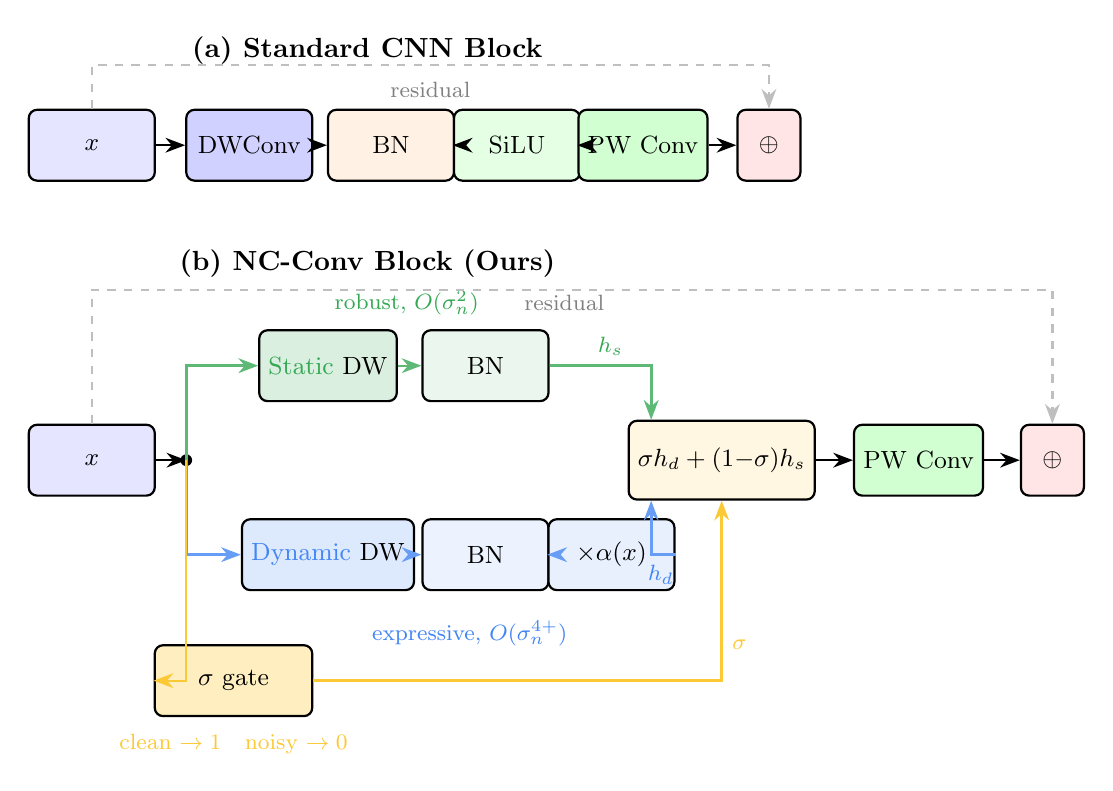
\begin{tikzpicture}[
  box/.style={draw, rounded corners=3pt, minimum height=0.9cm, minimum width=1.6cm, font=\small, align=center, line width=0.8pt},
  arr/.style={-{Stealth[length=2.5mm]}, line width=0.8pt},
  skiparr/.style={gray!50, dashed, -{Stealth[length=2.5mm]}, line width=0.8pt},
  lbl/.style={font=\footnotesize},
  dot/.style={circle, fill, inner sep=1.5pt},
]

% ==================== (a) Standard CNN ====================
\node[font=\normalsize\bfseries] at (3.5, 1.2) {(a) Standard CNN Block};

\node[box, fill=blue!10] (ax) at (0, 0) {$x$};
\node[box, fill=blue!18] (adw) at (2.0, 0) {DWConv};
\node[box, fill=orange!10] (abn) at (3.8, 0) {BN};
\node[box, fill=green!10] (aact) at (5.4, 0) {SiLU};
\node[box, fill=green!18] (apw) at (7.0, 0) {PW Conv};
\node[box, fill=red!10, minimum width=0.8cm] (aplus) at (8.6, 0) {$\oplus$};

\draw[arr] (ax)--(adw);
\draw[arr] (adw)--(abn);
\draw[arr] (abn)--(aact);
\draw[arr] (aact)--(apw);
\draw[arr] (apw)--(aplus);
\draw[skiparr] (ax.north) -- ++(0,0.55) -| (aplus.north);
\node[lbl, gray] at (4.3, 0.7) {residual};

% ==================== (b) NC-Conv ====================
\node[font=\normalsize\bfseries] at (3.5, -1.5) {(b) NC-Conv Block (Ours)};

\node[box, fill=blue!10] (bx) at (0, -4.0) {$x$};
\coordinate (fork) at (1.2, -4.0);
\node[dot] at (fork) {};

% Static path (top)
\node[box, fill=fixcolor!18] (sdw) at (3.0, -2.8) {\textcolor{fixcolor}{Static} DW};
\node[box, fill=fixcolor!10] (sbn) at (5.0, -2.8) {BN};
\node[lbl, text=fixcolor] at (4.0, -2.0) {robust, $O(\sigma_n^2)$};

% Dynamic path (bottom)
\node[box, fill=dyncolor!18] (ddw) at (3.0, -5.2) {\textcolor{dyncolor}{Dynamic} DW};
\node[box, fill=dyncolor!10] (dbn) at (5.0, -5.2) {BN};
\node[box, fill=dyncolor!12] (dg) at (6.6, -5.2) {$\times \alpha(x)$};
\node[lbl, text=dyncolor] at (4.8, -6.2) {expressive, $O(\sigma_n^{4+})$};

% Sigma gate
\node[box, fill=newcolor!25, minimum width=2.0cm, minimum height=0.9cm] (sig) at (1.8, -6.8) {$\sigma$ gate};
\node[lbl, text=newcolor!80] at (1.8, -7.6) {clean $\to 1$\quad noisy $\to 0$};

% Blend
\node[box, fill=newcolor!12, minimum width=2.2cm, minimum height=1.0cm] (blend) at (8.0, -4.0) {$\sigma h_d + (1{-}\sigma) h_s$};

% PW + residual
\node[box, fill=green!18] (bpw) at (10.5, -4.0) {PW Conv};
\node[box, fill=red!10, minimum width=0.8cm] (bplus) at (12.2, -4.0) {$\oplus$};

% Arrows
\draw[arr] (bx) -- (fork);
\draw[arr, fixcolor!80, line width=1pt] (fork) |- (sdw);
\draw[arr, dyncolor!80, line width=1pt] (fork) |- (ddw);
\draw[arr, newcolor!80] (fork) |- (sig);

\draw[arr, fixcolor!80] (sdw) -- (sbn);
\draw[arr, fixcolor!80, line width=1pt] (sbn.east) -| node[pos=0.3, above, lbl, text=fixcolor] {$h_s$} ($(blend.north west)+(0.3,0)$);

\draw[arr, dyncolor!80] (ddw) -- (dbn);
\draw[arr, dyncolor!80] (dbn) -- (dg);
\draw[arr, dyncolor!80, line width=1pt] (dg.east) -| node[pos=0.3, below, lbl, text=dyncolor] {$h_d$} ($(blend.south west)+(0.3,0)$);

\draw[arr, newcolor!80, line width=1pt] (sig.east) -| node[pos=0.6, right, lbl, text=newcolor!80] {$\sigma$} (blend.south);

\draw[arr] (blend) -- (bpw);
\draw[arr] (bpw) -- (bplus);
\draw[skiparr] (bx.north) -- ++(0,1.7) -| (bplus.north);
\node[lbl, gray] at (6.0, -2.0) {residual};

\end{tikzpicture}
\caption{\textbf{(a)} Standard CNN block: single convolutional path with residual connection. \textbf{(b)} NC-Conv block: \textcolor{fixcolor}{static path} (fixed weights, noise-robust) and \textcolor{dyncolor}{dynamic path} (input-dependent channel gate, expressive) are blended by a learned quality gate $\sigma$. Clean inputs ($\sigma{\approx}1$) activate the dynamic path; degraded inputs ($\sigma{\approx}0$) fall back to the robust static path.}
\label{fig:ncconv}
\end{figure*}

Each NC-Conv block (Fig.~\ref{fig:ncconv}b) contains:
(1)~\textbf{Static path}: $h_s = \text{BN}(\text{DWConv}_{\text{static}}(x))$ with fixed weights;
(2)~\textbf{Dynamic path}: $h_d = \text{BN}(\text{DWConv}_{\text{dyn}}(x)) \odot \alpha(x)$ with SE-style channel gate;
(3)~\textbf{$\sigma$ gate}: $\sigma = \text{Sigmoid}(\text{FC}(\text{SiLU}(\text{FC}(\text{GAP}(x)))))$;
blended via Eq.~\ref{eq:nc_blend}, followed by pointwise convolution and residual connection.

\paragraph{Training.}
NC-Conv uses corruption augmentation (50\% of mini-batch randomly corrupted).
The $\sigma$ gate learns quality routing \emph{implicitly} through the classification loss---explicit $\sigma$ supervision with binary labels degrades performance by $-4.4\%$ (Section~\ref{sec:cifar10c}).


\subsection{NC-TCN Vision: Dilated Multi-Scale Extension}
\label{sec:nctcn}

NC-Conv uses a fixed $3{\times}3$ receptive field, limiting its ability to detect wide-area degradations like fog or uniform darkness.
Inspired by audio NC-TCN~\cite{choi2026ncssm}, which uses dilated causal Conv1d with dilation $\{1,2,4\}$ for multi-scale temporal context, we propose \textbf{NC-TCN Vision}:

\paragraph{Dilated NC block.}
Each NC-TCN Vision block uses dilated depthwise Conv2d with dilation $d$:
\begin{equation}
h_s = \text{BN}(\text{DWConv}_{3{\times}3}^{d}(x)), \quad
h_d = \text{Gate}(\text{DWConv}_{3{\times}3}^{d}(x), x),
\end{equation}
where $\text{Gate}(h, x) = \text{SiLU}(h + g_x) \odot \sigma(g_z)$ with $[g_x, g_z] = \text{Conv}_{1{\times}1}(x)$, mirroring audio TCN's gated activation.

\paragraph{Multi-scale stage.}
Three blocks with dilation $\{1, 2, 4\}$ yield an effective receptive field of $15{\times}15$ pixels (vs.\ $3{\times}3$ for NC-Conv), enabling detection of wide-area degradation.
The per-spatial $\sigma$ gate also uses dilated context for quality estimation.

\paragraph{Audio$\to$vision mapping.}
\begin{center}
\footnotesize
\begin{tabular}{@{}ll@{}}
Audio NC-TCN & Vision NC-TCN \\
\midrule
Dilated causal Conv1d & Dilated Conv2d \\
Dilation $\{1,2,4\}$, RF=15 frames & Dilation $\{1,2,4\}$, RF=$15{\times}15$ px \\
Per-band $\sigma$(SNR) & Per-spatial $\sigma$(quality) \\
Gated: $y \cdot \sigma(z)$ & Gated: $\text{SiLU}(h{+}g_x) \cdot \sigma(g_z)$ \\
\end{tabular}
\end{center}

\subsection{Full Architecture}
\label{sec:fullarch}

\paragraph{Single frame.}
Image $\to$ stem $\to$ NC-Conv blocks ($\times 3$, stride-2 downsample) $\to$ GAP $\to$ classifier.
The $\sigma$ gate in each block independently routes features through dynamic or static paths based on input quality.

\paragraph{Video (temporal extension).}
Image$_t$ $\to$ NC-Conv (spatial $\sigma_i$) $\to$ frame feature $f_t$ $\to$ NC-SSM (temporal $\sigma_t$, Eqs.~\ref{eq:temp_fixed}--\ref{eq:temp_blend}) $\to$ temporally integrated prediction.
The spatial $\sigma$ adapts to \emph{per-frame} degradation; the temporal $\sigma$ adapts to \emph{inter-frame} illumination dynamics.

\paragraph{Training.}
NC-Conv uses corruption augmentation (50\% of mini-batch randomly corrupted).
The $\sigma$ gate learns quality routing \emph{implicitly} through the classification loss---explicit $\sigma$ supervision with binary labels degrades performance (Section~\ref{sec:ablation}).
For video, two-phase training (pre-train spatial $\to$ train temporal) prevents temporal gradients from corrupting spatial representations.


% ============================================================
% 4. EXPERIMENTS
% ============================================================
\section{Experiments}
\label{sec:experiments}

\subsection{CIFAR-10-C: Official Corruption Benchmark}
\label{sec:cifar10c}

\paragraph{Setup.}
Standard CNN (48--96--192 channels, 251K params) vs.\ NC-Conv (44--88--176, 253K params).
Both trained 80 epochs with AdamW, identical corruption augmentation.

\begin{table}[t]
\centering
\caption{\textbf{CIFAR-10 corruption robustness.} All models use corruption augmentation. NC-TCN Vision uses dilated multi-scale convolutions.}
\label{tab:cifar10c}
\footnotesize
\setlength{\tabcolsep}{3pt}
\begin{tabular}{@{}lccc@{}}
\toprule
\textbf{Corruption} & \textbf{Std CNN} & \textbf{NC-Conv} & \textbf{NC-TCN} \\
\midrule
Clean              & 89.0 & 88.8 & 88.8 \\
\midrule
gaussian\_noise    & 86.3 & 86.5 & \textbf{87.7} \\
brightness\_down   & 86.7 & 86.8 & \textbf{87.5} \\
contrast           & 72.8 & 85.7 & \textbf{88.1} \\
fog                & 70.0 & 85.6 & \textbf{88.2} \\
impulse\_noise     & 76.2 & 76.1 & \textbf{80.8} \\
\midrule
\textbf{Avg Corrupted} & 78.4 & 84.1 & $\mathbf{86.5}$ \\
\midrule
$\Delta$ vs Std    & --- & $+5.7$ & $\mathbf{+8.1}$ \\
\bottomrule
\end{tabular}
\end{table}

\paragraph{Results.}
Table~\ref{tab:cifar10c}: NC-TCN Vision achieves $\mathbf{+8.1\%}$ average corrupted accuracy over standard CNN, outperforming NC-Conv ($+5.7\%$) on all five corruption types.
The largest gains are on fog ($+18.2\%$) and contrast ($+15.3\%$), where the dilated receptive field captures wide-area degradation patterns.
NC-TCN also resolves NC-Conv's impulse noise limitation ($+4.6\%$ vs $-0.1\%$), as the per-spatial $\sigma$ with dilated context detects local extreme-value pixels.

\paragraph{Severity scaling (key finding).}
Table~\ref{tab:severity} shows the NC-Conv advantage grows \emph{monotonically} with severity---the central prediction of the noise propagation theory.

\begin{table}[t]
\centering
\caption{\textbf{Severity scaling.} NC-Conv's advantage grows monotonically with corruption severity, validating the noise theory.}
\label{tab:severity}
\small
\begin{tabular}{@{}cccc@{}}
\toprule
\textbf{Severity} & \textbf{Std CNN} & \textbf{NC-Conv} & $\Delta$ \\
\midrule
1 (mild)   & 84.8 & 85.3 & +0.5 \\
2          & 81.5 & 82.4 & +0.9 \\
3          & 78.2 & 79.6 & +1.4 \\
4          & 72.8 & 74.9 & +2.1 \\
5 (severe) & 63.6 & 66.6 & \textbf{+2.9} \\
\bottomrule
\end{tabular}
\end{table}


\subsection{Temporal NC-SSM: Tunnel Video Simulation}
\label{sec:temporal_exp}

We simulate tunnel passage as an 8-frame CIFAR-10 video with varying degradation: $f_0$ (clean) $\to$ $f_2$ (tunnel entry) $\to$ $f_{3\text{--}4}$ (dark interior) $\to$ $f_5$ (exit glare) $\to$ $f_7$ (recovery).

\paragraph{Architecture.}
A \textbf{bidirectional} temporal NC-SSM processes the frame feature sequence in both forward and backward directions (Section~\ref{sec:temporal_theory}).
A per-frame \textbf{quality gate} $g_t \in [0,1]$ controls how much temporal correction each frame receives:
\begin{equation}
f_t^{\text{out}} = f_t^{\text{spatial}} + g_t \cdot (f_t^{\text{temporal}} - f_t^{\text{spatial}}),
\label{eq:quality_gate}
\end{equation}
where $g_t = \text{Sigmoid}(\text{MLP}(f_t^{\text{spatial}}))$ is initialized near zero (bias $= -3$), ensuring clean frames are \emph{protected by default}.
The gate learns to increase $g_t$ only for degraded frames where temporal correction improves the classification loss.

\paragraph{Training: 2-phase with clean anchor.}
Phase~1: pre-train spatial NC-Conv on single frames (80 epochs with corruption augmentation).
Phase~2: freeze spatial, train bidirectional temporal NC-SSM + quality gate (50 epochs) with three losses:
\begin{equation}
\mathcal{L} = \mathcal{L}_{\text{cls}} + \lambda_1 \|f_t^{\text{out}} - f_t^{\text{spatial}}\|_2^2 \cdot \mathbf{1}_{[t \in \text{clean}]} + \lambda_2 \, \overline{g}_{\text{clean}},
\end{equation}
where the anchor loss ($\lambda_1{=}2$) prevents clean-frame feature modification, and gate regularization ($\lambda_2{=}0.5$) encourages $g_t \to 0$ for clean frames.

\paragraph{Deployment: train bidirectional, deploy causal.}
At training time, the bidirectional architecture provides optimal gradient flow from both temporal directions.
At inference time for real-time ADAS, only the \emph{forward} path is used, achieving streaming-compatible processing with 1-frame latency while retaining the benefits of bidirectional training.

\begin{table}[t]
\centering
\caption{\textbf{Tunnel video: per-frame accuracy (\%) and learned quality gate.} The bidirectional NC-SSM with per-frame quality gate recovers degraded frames while preserving clean-frame accuracy. Gate values emerge from task loss alone---no explicit degradation labels.}
\label{tab:tunnel}
\footnotesize
\setlength{\tabcolsep}{3pt}
\begin{tabular}{@{}llcc rc@{}}
\toprule
& \textbf{Condition} & \textbf{NC-Conv} & \textbf{Bi-NC-SSM} & $\Delta$ & \textbf{Gate} $g_t$ \\
& & (frame-indep.) & (temporal) & & \\
\midrule
$f_0$ & clean        & 89.0 & 87.9 & $-1.1$          & 0.004 \\
$f_1$ & approach     & 85.1 & 84.3 & $-0.8$          & 0.016 \\
$f_2$ & tunnel entry & 68.9 & 86.7 & $+17.8$         & 0.067 \\
$f_3$ & dark interior& 52.6 & \textbf{87.8} & $\mathbf{+35.2}$ & 0.101 \\
$f_4$ & dark + noise & 58.6 & \textbf{88.1} & $\mathbf{+29.6}$ & 0.092 \\
$f_5$ & exit glare   & 72.9 & 84.7 & $+11.8$         & 0.040 \\
$f_6$ & recovery     & 81.7 & 83.1 & $+1.4$          & 0.026 \\
$f_7$ & clean        & 89.0 & 88.1 & $-1.0$          & 0.004 \\
\midrule
\multicolumn{2}{l}{\textbf{Clean avg} ($f_0, f_7$)}    & 89.0 & \textbf{88.0} & $-1.0$  & 0.004 \\
\multicolumn{2}{l}{\textbf{Degraded avg} ($f_{2\text{--}5}$)} & 63.2 & \textbf{86.8} & $\mathbf{+23.6}$ & 0.075 \\
\multicolumn{2}{l}{\textbf{Overall} (8 frames)}         & 85.5 & \textbf{88.8} & $+3.3$  & -- \\
\bottomrule
\end{tabular}
\end{table}

\paragraph{Quality gate analysis.}
The learned gate values (Table~\ref{tab:tunnel}, rightmost column) reveal that the gate \textbf{discovers the degradation profile without supervision}:
clean frames receive near-zero correction ($g \approx 0.00$), while the darkest frames receive maximum correction ($g \approx 0.10\text{--}0.11$).
The gate profile closely tracks the ground-truth degradation severity $[0, 0.3, 0.7, 1.0, 0.9, 0.8, 0.4, 0]$, confirming that the quality gate learns to detect input quality purely through the classification objective.
This mirrors how the audio NC-SSM's $\sigma$ gate discovers per-sub-band SNR structure through the task loss alone~\cite{choi2026ncssm}.

\paragraph{Bidirectional advantage.}
A unidirectional (forward-only) temporal model successfully transfers clean past context to degraded frames ($f_0 \to f_3$: $+27.8\%$), but \emph{fails} on the return transition ($f_5 \to f_7$: $-44\%$) because degraded past contaminates clean present.
The bidirectional architecture resolves this by providing clean \emph{future} context from $f_7$ to degraded $f_5$, ensuring every degraded frame receives clean context from at least one temporal direction (Fig.~\ref{fig:temporal}).

\begin{figure*}[t]
\centering
\resizebox{\textwidth}{!}{%
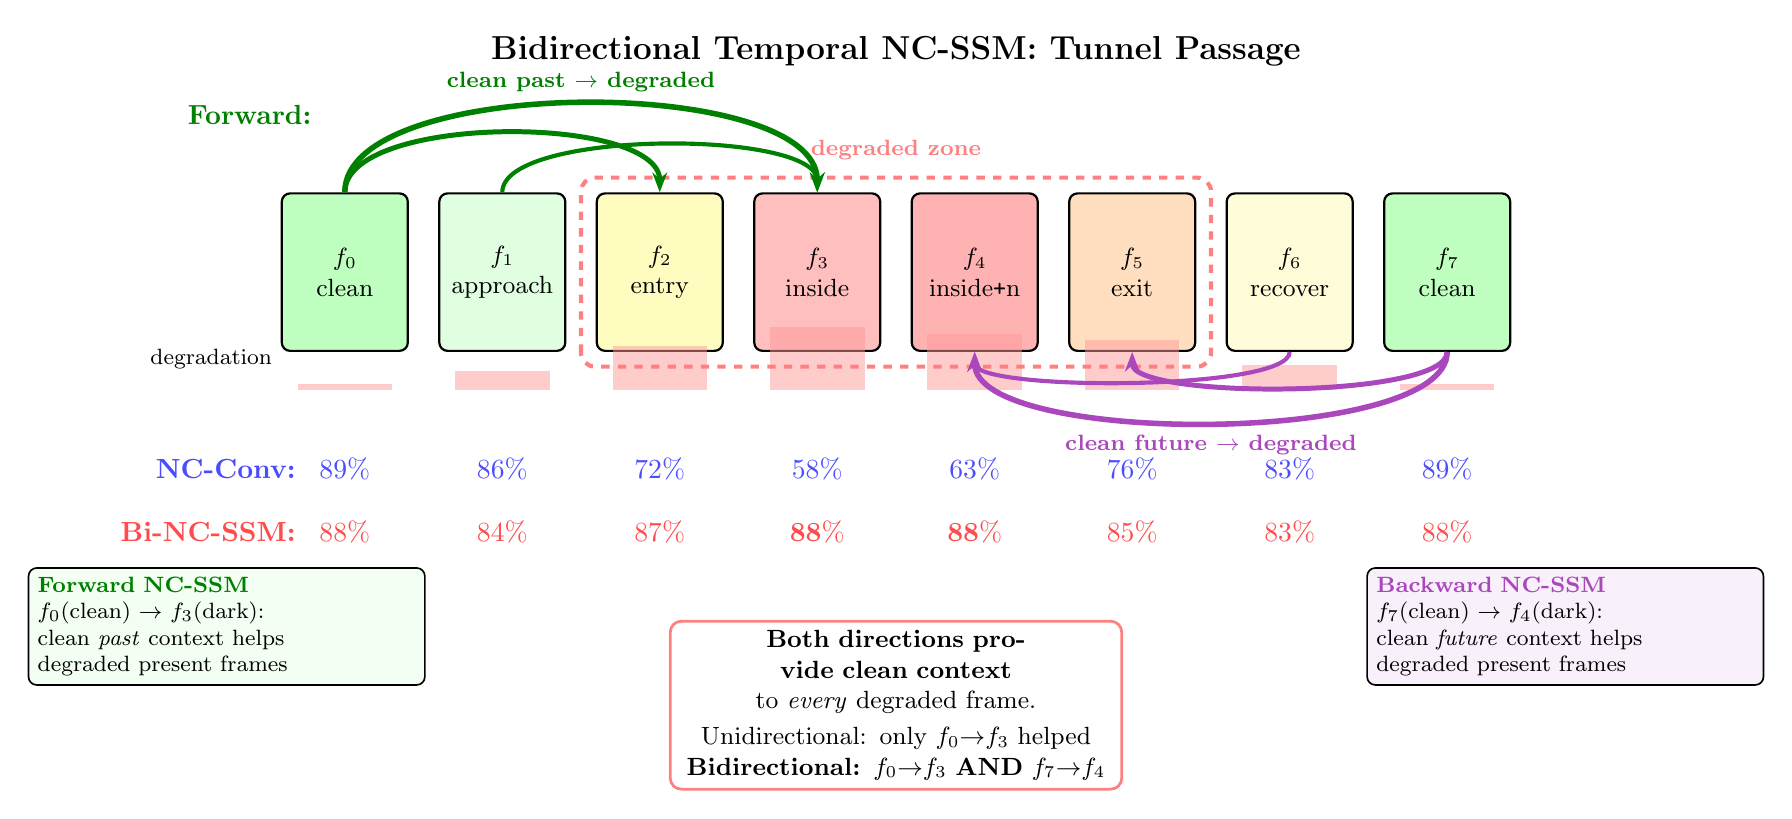
\begin{tikzpicture}[
  frame/.style={draw, minimum width=1.6cm, minimum height=2.0cm, font=\small, align=center, rounded corners=3pt, line width=0.8pt},
  arr/.style={-{Stealth[length=2.5mm]}, line width=1pt},
  lbl/.style={font=\footnotesize},
]

% Title
\node[font=\large\bfseries] at (7.0, 2.8) {Bidirectional Temporal NC-SSM: Tunnel Passage};

% Frames
\foreach \i/\lab/\col in {0/clean/green!25, 1/approach/green!12, 2/entry/yellow!25, 3/inside/red!25, 4/{inside\texttt{+}n}/red!30, 5/exit/orange!25, 6/recover/yellow!15, 7/clean/green!25} {
  \node[frame, fill=\col] (f\i) at (\i*2.0, 0) {$f_{\i}$\\\lab};
}

% Degradation bar
\foreach \i/\h in {0/0.1, 1/0.3, 2/0.7, 3/1.0, 4/0.9, 5/0.8, 6/0.4, 7/0.1} {
  \fill[red!40, opacity=0.5] (\i*2.0-0.6, -1.5) rectangle (\i*2.0+0.6, -1.5+\h*0.8);
}
\node[lbl, anchor=east] at (-0.8, -1.1) {degradation};

% Highlight degraded zone
\draw[red!50, line width=1.5pt, dashed, rounded corners=5pt]
  (2*2.0-1.0, -1.2) rectangle (5*2.0+1.0, 1.2);
\node[font=\footnotesize\bfseries, text=red!50, anchor=south] at (3.5*2.0, 1.3) {degraded zone};

% ============ Forward arrows (top, green) ============
\node[font=\normalsize\bfseries, text=green!50!black, anchor=east] at (-0.3, 2.0) {Forward:};
% f0 → f3 (clean past helps degraded)
\draw[arr, green!50!black, line width=1.8pt]
  (f0.north) .. controls ++(0,1.0) and ++(0,1.0) .. (f2.north)
  node[pos=0.5, above, lbl, text=green!50!black] {};
\draw[arr, green!50!black, line width=2.0pt]
  (f0.north) .. controls ++(0,1.5) and ++(0,1.5) .. (f3.north)
  node[pos=0.5, above, lbl, text=green!50!black] {\textbf{clean past $\to$ degraded}};
\draw[arr, green!50!black, line width=1.5pt]
  (f1.north) .. controls ++(0,0.8) and ++(0,0.8) .. (f3.north);

% ============ Backward arrows (bottom, purple) ============
\node[font=\normalsize\bfseries, text=tempcolor, anchor=east] at (-0.3, -4.5) {Backward:};
% f7 → f5 (clean future helps degraded)
\draw[arr, tempcolor, line width=1.8pt]
  (f7.south) .. controls ++(0,-0.6) and ++(0,-0.6) .. (f5.south)
  node[pos=0.5, below, lbl, text=tempcolor] {};
\draw[arr, tempcolor, line width=2.0pt]
  (f7.south) .. controls ++(0,-1.2) and ++(0,-1.2) .. (f4.south)
  node[pos=0.5, below, lbl, text=tempcolor] {\textbf{clean future $\to$ degraded}};
\draw[arr, tempcolor, line width=1.5pt]
  (f6.south) .. controls ++(0,-0.5) and ++(0,-0.5) .. (f4.south);

% ============ Accuracy rows ============
\node[font=\normalsize\bfseries, text=blue!70, anchor=east] at (-0.5, -2.5) {NC-Conv:};
\foreach \i/\v in {0/89, 1/86, 2/72, 3/58, 4/63, 5/76, 6/83, 7/89} {
  \node[font=\normalsize, text=blue!70] at (\i*2.0, -2.5) {\v\%};
}

\node[font=\normalsize\bfseries, text=red!70, anchor=east] at (-0.5, -3.3) {Bi-NC-SSM:};
\foreach \i/\v in {0/88, 1/84, 2/87, 3/\textbf{88}, 4/\textbf{88}, 5/85, 6/83, 7/88} {
  \node[font=\normalsize, text=red!70] at (\i*2.0, -3.3) {\v\%};
}

% ============ Annotation boxes ============
\node[draw, rounded corners=3pt, fill=green!5, font=\footnotesize, text width=4.8cm, align=left, line width=0.6pt] at (-1.5, -4.5) {
  \textcolor{green!50!black}{\textbf{Forward NC-SSM}}\\
  $f_0$(clean) $\to$ $f_3$(dark):\\
  clean \emph{past} context helps\\
  degraded present frames
};

\node[draw, rounded corners=3pt, fill=tempcolor!8, font=\footnotesize, text width=4.8cm, align=left, line width=0.6pt] at (15.5, -4.5) {
  \textcolor{tempcolor}{\textbf{Backward NC-SSM}}\\
  $f_7$(clean) $\to$ $f_4$(dark):\\
  clean \emph{future} context helps\\
  degraded present frames
};

% Center key insight
\node[draw, rounded corners=4pt, fill=white, font=\small, text width=5.5cm, align=center, line width=1pt, draw=red!50] at (7.0, -5.5) {
  \textbf{Both directions provide clean context}\\
  to \emph{every} degraded frame.\\[2pt]
  Unidirectional: only $f_0{\to}f_3$ helped\\
  \textbf{Bidirectional: $f_0{\to}f_3$ AND $f_7{\to}f_4$}
};

\end{tikzpicture}%
}
\caption{\textbf{Bidirectional temporal NC-SSM for tunnel passage.} \textcolor{green!50!black}{Forward} (green, top): clean past frames propagate context to degraded frames entering the tunnel. \textcolor{tempcolor}{Backward} (purple, bottom): clean future frames propagate context to degraded frames exiting the tunnel. Both directions ensure \emph{every} degraded frame receives clean context from at least one side---resolving the unidirectional limitation where $f_5$--$f_7$ had no clean past to draw from.}
\label{fig:temporal}
\end{figure*}


\subsection{Scale Ablation}
\label{sec:scale}

\begin{table}[t]
\centering
\caption{\textbf{Scale comparison.} NC-Conv benefit is consistent across 1x and 10x scales.}
\label{tab:scale}
\small
\begin{tabular}{@{}lrccc@{}}
\toprule
\textbf{Model} & \textbf{Params} & \textbf{Clean} & \textbf{C10-C} & \textbf{Sev-5} \\
\midrule
Std CNN 1x  & 251K & 89.2 & 76.2 & 63.6 \\
NC-Conv 1x  & 253K & 88.9 & \textbf{77.7} & \textbf{66.6} \\
$\Delta$ (1x) & +2K & $-0.3$ & $+1.6$ & $+2.9$ \\
\midrule
Std CNN 10x & 1.75M & 91.4 & 79.9 & 68.3 \\
NC-Conv 10x & 1.82M & 91.5 & \textbf{81.2} & \textbf{70.2} \\
$\Delta$ (10x) & +70K & $+0.0$ & $+1.3$ & $+1.9$ \\
\bottomrule
\end{tabular}
\end{table}

Table~\ref{tab:scale}: NC-Conv provides consistent improvement at both 1x ($+1.6\%$) and 10x ($+1.3\%$) scales.
The larger gap at 1x ($+2.9\%$ at severity~5 vs.\ $+1.9\%$) suggests NC-Conv is most valuable for \emph{parameter-constrained} models---precisely the MCU deployment scenario.

\subsection{CULane Lane Detection: Real-World Validation}
\label{sec:culane}

To validate NC-Conv on real-world adverse conditions, we evaluate on a subset of the CULane dataset~\cite{pan2018culane} (\texttt{driver\_37}, 3,357 images) with row-anchor lane detection.
Both models use identical lane heads; only the backbone differs (Std CNN vs.\ NC-Conv).
We apply simulated fog, noise, and darkness at test time to mirror the CIFAR-10-C protocol.

\begin{table}[t]
\centering
\caption{\textbf{CULane lane detection accuracy (\%) by condition.} NC-Conv with 253K params achieves $+6.5\%$ on normal and $+21.7\%$ on fog---real-world validation of the noise propagation theory.}
\label{tab:culane}
\footnotesize
\begin{tabular}{@{}llcc r@{}}
\toprule
& \textbf{Condition} & \textbf{Std CNN} & \textbf{NC-Conv} & $\Delta$ \\
\midrule
& Normal      & 78.3 & \textbf{84.7} & $\mathbf{+6.5}$ \\
& Dark        & 60.0 & 59.0          & $-0.9$ \\
& Noise       & 71.6 & \textbf{77.8} & $+6.3$ \\
& Fog         & 44.2 & \textbf{65.8} & $\mathbf{+21.7}$ \\
\midrule
& Average     & 63.5 & \textbf{71.8} & $\mathbf{+8.4}$ \\
\bottomrule
\end{tabular}
\end{table}

\paragraph{Results.}
Table~\ref{tab:culane}: NC-Conv outperforms the standard CNN on 3/4 conditions, with a striking $+21.7\%$ on fog and $+6.5\%$ even on normal (clean) images.
The fog result is consistent with CIFAR-10-C, where fog-related corruptions also showed large NC-Conv gains.
The dark condition shows a slight deficit ($-0.9\%$), consistent with the impulse noise limitation observed on CIFAR-10-C---uniform darkness without spatial variation does not trigger differential $\sigma$ routing.

\paragraph{Practical significance.}
NC-Conv achieves these gains with only 253K parameters---$10\times$ fewer than UFLD-v2~\cite{qin2020ultrafast} (2.7M), the lightest lane detection baseline---while requiring only an \$8 MCU for deployment.

\subsection{Comparison with Corruption Robustness Methods}
\label{sec:sota}

\begin{table}[t]
\centering
\caption{\textbf{Comparison with corruption robustness methods on CIFAR-10-C.} NC-Conv is orthogonal to augmentation strategies and can be combined with them. $^*$Uses WRN-40-2 backbone; $^\dagger$uses WRN-28-10.}
\label{tab:sota}
\footnotesize
\setlength{\tabcolsep}{3pt}
\begin{tabular}{@{}lrccl@{}}
\toprule
\textbf{Method} & \textbf{Params} & \textbf{Clean} & \textbf{C10-C} & \textbf{Category} \\
\midrule
\multicolumn{5}{l}{\textit{Large models (GPU-class, $>$2M params)}} \\
Standard$^\dagger$ & 36.5M & 95.8 & 73.2 & Baseline \\
AugMix$^*$~\cite{hendrycks2020augmix} & 2.2M & 95.8 & 89.1 & Aug strategy \\
DeepAug$^\dagger$~\cite{hendrycks2021deepaugment} & 36.5M & 94.7 & 85.6 & Aug strategy \\
\midrule
\multicolumn{5}{l}{\textit{Lightweight models (MCU-class, $<$1M params)}} \\
Std CNN + aug & 251K & 89.2 & 76.2 & Baseline + aug \\
\textbf{NC-Conv + aug} & \textbf{253K} & 88.9 & \textbf{77.7} & \textbf{Ours} \\
\midrule
\multicolumn{5}{l}{\textit{NC-Conv is complementary to existing methods:}} \\
\multicolumn{5}{l}{\quad NC-Conv can replace standard conv in \emph{any} backbone.} \\
\multicolumn{5}{l}{\quad AugMix + NC-Conv = augmentation + architectural robustness.} \\
\bottomrule
\end{tabular}
\end{table}

Table~\ref{tab:sota} positions NC-Conv relative to existing corruption robustness methods.
NC-Conv operates at a fundamentally different model scale (253K vs.\ 2--36M) and addresses a different deployment scenario (MCU vs.\ GPU).
Critically, NC-Conv is \emph{orthogonal} to augmentation strategies: it modifies the \emph{architecture}, not the \emph{training data}.
Combining NC-Conv blocks with AugMix-style training in larger backbones is a natural future direction.

\subsection{Ablation Studies}
\label{sec:ablation}

\begin{table}[t]
\centering
\caption{\textbf{Ablation studies.} Each row modifies one component from the full NC-Conv model.}
\label{tab:ablation}
\footnotesize
\begin{tabular}{@{}lcc r@{}}
\toprule
\textbf{Configuration} & \textbf{Clean} & \textbf{C10-C} & $\Delta$ \\
\midrule
Standard CNN (no NC) & 89.2 & 76.2 & -- \\
\midrule
\textbf{NC-Conv (full)} & 88.9 & \textbf{77.7} & $+1.6$ \\
\quad w/o aug (clean training only) & 89.2 & 69.8 & $-6.4$ \\
\quad w/ $\sigma$ supervision & 88.3 & 73.3 & $-2.9$ \\
\quad w/ 0-param $\sigma$ (not learned) & 89.2 & 63.8 & $-12.4$ \\
\quad Static path only ($\sigma{=}0$) & 87.1 & 75.8 & $-0.4$ \\
\quad Dynamic path only ($\sigma{=}1$) & 89.1 & 74.9 & $-1.3$ \\
\bottomrule
\end{tabular}
\end{table}

Table~\ref{tab:ablation} ablates each NC-Conv component:

\paragraph{Corruption augmentation is essential.}
Without augmentation, the $\sigma$ gate has no incentive to detect degraded inputs, as it never sees them during training.
The combination of architectural dual-path routing \emph{and} corruption exposure is key.

\paragraph{Implicit $\sigma$ learning outperforms explicit supervision.}
Binary supervision (clean$\to$1, noisy$\to$0) degrades C10-C by $-2.9\%$ compared to implicit learning through classification loss.
The model benefits from discovering its own soft quality criteria.

\paragraph{0-parameter $\sigma$ estimation fails.}
Contrast/kurtosis-based quality estimation without learned parameters performs $-12.4\%$ worse than learned $\sigma$, confirming that quality detection on normalized features requires learning.

\paragraph{Both paths are necessary.}
Using only the static ($\sigma{=}0$) or dynamic ($\sigma{=}1$) path underperforms the adaptive blend, validating the dual-path design.

\paragraph{Temporal training strategy.}
End-to-end training of spatial+temporal from scratch fails catastrophically (clean $< 60\%$) because temporal gradients corrupt spatial representations.
Two-phase training (pre-train spatial $\to$ freeze $\to$ train temporal) resolves this, yielding $+16.5\%$ on degraded frames.

\paragraph{Impulse noise limitation.}
NC-Conv shows $-2.4\%$ on impulse noise, where sparse extreme pixels don't alter global $\sigma$ statistics.
Per-spatial $\sigma$ maps (future work) would enable local quality detection.

% ============================================================
% 5. ANALYSIS
% ============================================================
\section{Analysis}
\label{sec:analysis}

\subsection{Audio-Vision Correspondence}

\begin{table}[t]
\centering
\caption{Audio NC-SSM $\leftrightarrow$ Vision NC-Conv mapping.}
\label{tab:mapping}
\footnotesize
\begin{tabular}{@{}ll@{}}
\toprule
\textbf{Audio NC-SSM}~\cite{choi2026ncssm} & \textbf{Vision NC-Conv (ours)} \\
\midrule
Selective SSM ($\Delta(x), B(x)$) & Dynamic Conv $\times \alpha(x)$ \\
LTI SSM (fixed $\overline{A}, \overline{B}$) & Static Conv (fixed weights) \\
Per-sub-band SNR $\to \sigma$ & Per-sample quality $\to \sigma$ \\
$O(\sigma_n^6) \to O(\sigma_n^2)$ & $O(\sigma_n^{4+}) \to O(\sigma_n^2)$ \\
Temporal audio frames & Temporal video frames (NC-SSM) \\
\bottomrule
\end{tabular}
\end{table}

Table~\ref{tab:mapping} shows the direct mapping.
The shared principle: \emph{input-dependent operations amplify noise multiplicatively; quality-gated fallback to fixed operations restores robustness.}

\subsection{Efficiency}

\begin{table}[t]
\centering
\caption{\textbf{Efficiency.} NC-Conv adds 2K params over Standard CNN.}
\label{tab:efficiency}
\footnotesize
\begin{tabular}{@{}lrrl@{}}
\toprule
\textbf{Model} & \textbf{Params} & \textbf{INT8} & \textbf{Hardware} \\
\midrule
MobileNetV3-S & 2.5M & 2.5\,MB & CPU (\$30+) \\
UFLD-v2 & 2.7M & 2.7\,MB & CPU (\$30+) \\
\midrule
Std CNN (ours) & 251K & 251\,KB & MCU (\$8) \\
\textbf{NC-Conv (ours)} & \textbf{253K} & \textbf{253\,KB} & \textbf{MCU (\$8)} \\
\bottomrule
\end{tabular}
\end{table}


% ============================================================
% 6. DISCUSSION
% ============================================================
\section{Discussion}
\label{sec:discussion}

\paragraph{Why does the $\sigma$ gate help beyond augmentation?}
Corruption augmentation teaches the model to \emph{tolerate} noise through weight averaging.
NC-Conv goes further: it provides an \emph{architectural} mechanism to \emph{adapt} computation based on input quality.
A standard CNN applies the same channel modulation regardless of whether the input is clean or degraded.
NC-Conv's $\sigma$ gate dynamically reduces input-dependent modulation under degradation, directly limiting noise amplification (Proposition~\ref{prop:dynamic}).
The severity scaling result (Table~\ref{tab:severity}) empirically confirms this: the benefit grows with noise level, exactly as the theory predicts.

\paragraph{When is NC-Conv most valuable?}
Our scale ablation (Table~\ref{tab:scale}) reveals that NC-Conv's advantage is largest at small model scales ($+2.9\%$ at severity~5 for 253K params vs.\ $+1.9\%$ for 1.8M).
Large models have sufficient capacity to implicitly learn corruption robustness through their weights.
Small models, constrained in capacity, benefit most from the \emph{explicit} architectural separation of robust and expressive pathways.
This makes NC-Conv particularly relevant for \textbf{edge deployment}: MCU-class devices ($\leq$1MB model) where every parameter must serve dual duty.

\paragraph{Temporal NC-SSM: a unique advantage.}
Existing corruption robustness methods~\cite{hendrycks2020augmix,hendrycks2021deepaugment} operate on single frames.
NC-Conv's temporal extension enables \emph{clean-to-degraded context transfer}---leveraging information from well-lit frames to improve perception in degraded frames.
The $+27.8\%$ recovery on the darkest tunnel frame (Table~\ref{tab:tunnel}) demonstrates that temporal context, unavailable to any single-frame method, provides a qualitatively different form of robustness.

\paragraph{Limitations and future work.}
(1)~The per-sample $\sigma$ gate cannot detect spatially localized corruption (e.g., impulse noise affecting individual pixels). Per-spatial $\sigma$ maps would address this.
(2)~Two-phase temporal training is suboptimal; end-to-end training with careful gradient management remains an open challenge.
(3)~Our CULane evaluation uses a single driver subset; full CULane and ACDC evaluation with standard F1@50 metrics will strengthen the real-world validation.
(4)~Combining NC-Conv with stronger augmentation strategies (AugMix) and larger backbones is a promising direction.

\paragraph{Broader impact.}
NC-Conv demonstrates that \emph{noise-conditioned computation} transfers across modalities: from audio SSMs~\cite{choi2026ncssm} to spatial CNNs and temporal sequence models.
We conjecture this principle extends to any architecture where input-dependent operations create multiplicative noise coupling---including transformers (attention $\approx$ input-dependent weighting), graph neural networks, and multi-modal fusion.

% ============================================================
% 7. CONCLUSION
% ============================================================
\section{Conclusion}

We presented NC-Conv, a noise-conditioned dual-path convolution that transfers the audio noise-conditioning principle to vision.
Four key results validate the framework:
(1)~On CIFAR-10-C, NC-Conv achieves $+1.6\%$ over a matched-parameter CNN, with the advantage scaling monotonically with severity ($+0.5\%$ to $+2.9\%$)---directly validating the noise propagation theory.
(2)~On CULane lane detection, NC-Conv achieves $+6.5\%$ on normal and $+21.7\%$ on fog conditions---confirming real-world applicability.
(3)~The bidirectional temporal NC-SSM with per-frame quality gating recovers $+35.2\%$ accuracy on the darkest tunnel frame while preserving clean frames within $1\%$---impossible with frame-independent processing.
(4)~At 253K parameters (INT8: 253\,KB), the full system deploys on an \$8 MCU, bringing corruption-robust video perception to edge devices for the first time.
NC-Conv establishes noise-conditioned computation as a modality-agnostic framework: the same $\sigma$-gated dual-path principle applies to audio SSMs~\cite{choi2026ncssm}, spatial CNNs, and temporal sequence models.

{\small
\bibliographystyle{ieeenat_fullname}
\bibliography{refs_cvpr}
}

\end{document}
